\documentclass[11pt]{report}

%% ============================================================
%% Document Class and Basic Configuration
%% ============================================================
\usepackage{SNUformat}

% Define document information
% INFORMATION
\def\tNameKor{{홍길동}}
\def\tNameEng{{Hong Gil Dong}}
\def\tStudentNumber{2000-12345}

\def\tTitleKorean{{한국어 제목}}
\def\tTitleEnglish{{PUT YOUR ENGLISH TITLE HERE}}

% KOREAN
\def\tDepartmentKorean{{지구환경과학부}}
\def\tDateKorean{{2025년 2월}}

% ENGLISH
\def\tDepartmentEnglish{{Graduate School of Earth and Environmental Sciences}}
\def\tDate{{February 2025}}

%% ============================================================
%% Begin Document
%% ============================================================
\begin{document}

%% ============================================================
%% COVER PAGE
%% ============================================================
% DO NOT show page numbering
\pagestyle{empty}

\begin{titlepage}

    % Title Page.
    \renewcommand{\baselinestretch}{1}
    \centering
    {\Large \quad \par}
    \vspace{.5cm}

    % MAIN PAGE
    % Ph.D. Dissertation vs. Ph.D. Dissertation of "Natural Sciences"
    % 1: Proposal
    % {\fontsize{14}{0}\selectfont Research Proposal for a Ph.D. Thesis \par}
    
    % 2: Dissertation
    % Choose the appropriate line below based on your document type.
    % {\fontsize{14}{14pt}\selectfont \textbf{Ph.D. Dissertation of Natural Science} \par}
    {\fontsize{14}{14pt}\selectfont \textbf{이학박사 학위논문} \par}

    %% ============================
    %% TITLE (제목)
    %% ============================
    \vspace{1.5cm}
    {\fontsize{18}{27pt}\selectfont \textbf{\tTitleEnglish} \par}
    \vspace{1cm}
    {\fontsize{18}{27pt}\selectfont \textbf{\tTitleKorean} \par}
    
    %% ============================
    %% DATE for dissertation
    %% ============================
    \vfill % rather than using vspace, vfill is more effective.
    {\fontsize{16}{16pt}\selectfont \textbf{\tDate} \par}
    % or you can manually specify the Korean date as well.
    % {\fontsize{14}{14pt}\selectfont \textbf{2025년 2월} \par}

    %% ============================
    %% AFFILIATION AND AUTHOR in KOREAN
    %% ============================
    \vspace{3cm}
    {\fontsize{16}{16pt}\selectfont \textbf{서울대학교 대학원} \par}
    \vspace{.5cm}
    {\fontsize{16}{16pt}\selectfont \textbf{\tDepartmentKorean} \par}
    \vspace{.5cm}
    % {\fontsize{16}{16pt}\selectfont \textbf{Natural Science} \par}
    % \vspace{.5cm}
    {\fontsize{16}{16pt}\selectfont  \textbf{\tNameKor} \par}

    %% ============================
    %% AFFILIATION AND AUTHOR in ENGLISH
    %% ============================
    % {\fontsize{16}{16pt}\selectfont \textbf{\DepartmentEnglish} \par}
    % \vspace{.5cm}
    % {\fontsize{16}{16pt}\selectfont \textbf{Seoul National University} \par}
    % \vspace{.5cm}
    % {\fontsize{16}{16pt}\selectfont  \textbf{\tNameEng} \par}

\end{titlepage}

%% ============================================================
%% Title Page and Certificate Inclusion
%% ============================================================
% Add 인준지
% frame=true % for debugging
% scale=0.8
% offset=0cm 1cm % x: 0cm 변경 없음/ y: 1cm 위로 이동
\newpage
% Initialize the approval sheet inclusion
\clearpage

% put the approval sheet content here
\begin{center}
    
{\Large \quad \par}
\vspace{.1cm}
{\fontsize{20}{30bp}\selectfont \tTitleEnglish \par}
% {\Huge \tTitleA \par}
% \vspace{1.2cm}
\vfill
{\Large 지도교수 $\ $ 홍 $\ $ 길 $\ $ 동 \par}
\vspace{1cm}
{\Large 이 논문을 이학박사 학위논문으로 제출함 \par}
\vspace{.2cm}
{\Large \tDate \par}

\vspace{.9cm}
{\Large 서울대학교 대학원 \par}
\vspace{.2cm}
{\Large \tDepartmentKorean \par}
\vspace{.2cm}
{\Large \tNameKor \par}
\vspace{.9cm}

{\Large \tNameKor의 박사 학위논문을 인준함 \par}
\vspace{.1cm}
{\Large \tDate \par}

\vspace{1.2cm}
{\Large 위\hspace{.255cm}원\hspace{.255cm}장} \quad {\Large \underline{\qquad\qquad\qquad\qquad\qquad(인)} } \par
\vspace{.3cm}
{\Large 부위원장} \quad {\Large \underline{\qquad\qquad\qquad\qquad\qquad(인)} } \par
\vspace{.3cm}
{\Large 위\hspace{1cm}원} \quad {\Large \underline{\qquad\qquad\qquad\qquad\qquad(인)} } \par
\vspace{.3cm}
{\Large 위\hspace{1cm}원} \quad {\Large \underline{\qquad\qquad\qquad\qquad\qquad(인)} } \par
\vspace{.3cm}
{\Large 위\hspace{1cm}원} \quad {\Large \underline{\qquad\qquad\qquad\qquad\qquad(인)} } \par 

\end{center}
% NOTE: If you have approval sheet (인준지), include it using the "includepdf" instead of "input"
% 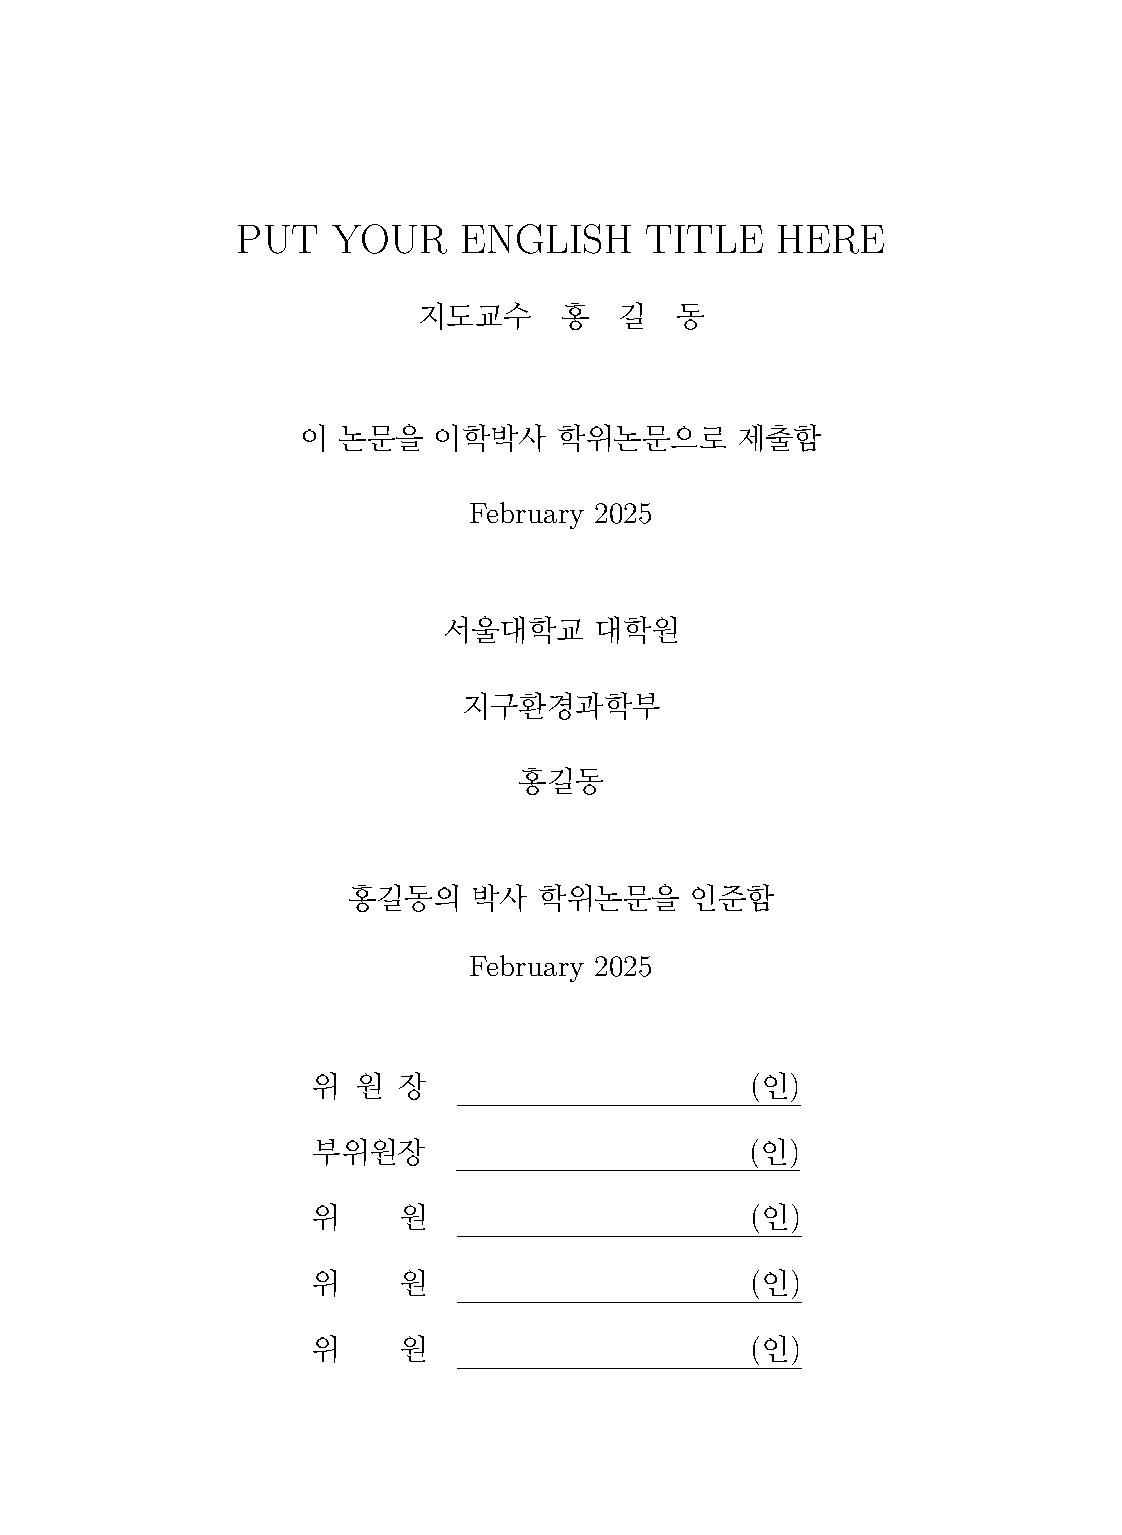
\includepdf[frame=false, % for debuggging
%         width=\paperwidth,
%         offset=0cm -1.5cm]{./templates/approval_sheet.pdf}

%% ============================================================
%% Abstract Section
%% ============================================================
\newpage
\pagestyle{plain} % resume page numbering
\pagenumbering{roman} % page numbering in ROMAN style : e.g., i, ii, iii, iv, ...
\begin{abstract}\addcontentsline{toc}{chapter}{Abstract}
    \setcounter{page}{1}

    % Write your abstract content here. Summarize the key objectives, methods, results, and conclusions of your research.

    % show dummy contents
    \lipsum[1]

\vfill
\noindent{\textbf{Key words}: PUT YOUR KEYWORDS}

\noindent{\textbf{Student Number}: \tStudentNumber}
\end{abstract}

%% ============================================
%% IMPORTANT: Reset page counter for main content
%% \begin{abstract} ... \end{abstract} does not count towards the main content page numbering, so we reset the page counter here.
%% ============================================
\setcounter{page}{2}

% ============================================================
% Table of contents, list of figures, and list of tables
% ============================================================
{
\setstretch{1}
\tableofcontents
\listoffigures
\listoftables
}

\newpage
%% ============================================================
%% Start of main content chapters
%% ============================================================
% Turn-on Arabic page numbering for main content chapters
\pagenumbering{arabic}

% Chapter 1: introduction
\chapter{Introduction}\label{c:chp1}

% Dummy text for demonstration purposes
\lipsum[1]

\section{Section 1.1}

\subsection{Section 1.1.1}

\subsubsection{Section 1.1.1.1}

\paragraph{Paragraph 1.1.1.1.1}

\subparagraph{Paragraph 1.1.1.1.1.1}

% Chapter 2
\chapter{TITLE OF CHAPTER 2}\label{c:chp2}
% \footnotetext{PUT YOUR FOOTNOTE TEXT HERE}


\section{Example: Equation}

Example for equation

\begin{lstlisting}[language=TeX]
    \begin{equation}\label{eq:einstein}
        E = mc^2
    \end{equation}
\end{lstlisting}

\begin{equation}\label{eq:einstein}
    E = mc^2
\end{equation}


Using \verb|\ref{eq:einstein}| will produce the equation number for Einstein's famous equation: \ref{eq:einstein}.

\section{Example: Citation}

This template uses the "natbib" package for handling citations.

\verb|\citet{morlighem2010spatial}| : \citet{morlighem2010spatial}

\verb|\citep{morlighem2010spatial}| : \citep{morlighem2010spatial}

\section{Example: Use Acronyms}

Here is an example of how to use acronyms defined with the ``acro'' package.
For instance, the acronym for ``Artificial Intelligence'' can be used as follows:

First use the acronym with \verb|\ac{AI}|: \ac{AI}.

Second use the acronym with \verb|\ac{AI}| again: \ac{AI}.

\verb|\acs{AI}| : Force the AI acronym to be plural: \acs{AI}


\subsection{Example: Figures and Tables}

First, include the figure using following command in your LaTeX document:

\begin{lstlisting}[language=TeX]
\begin{figure}
\centering
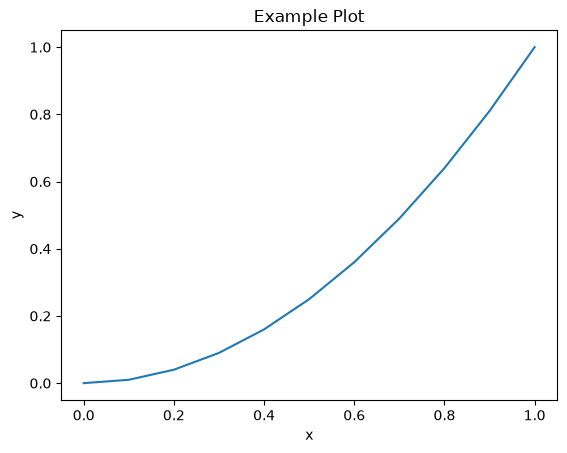
\includegraphics[width=1.0\textwidth]{Figures/Fig_Example.png}
\caption{PUT YOUR CAPTON}
\label{fig:example}
\end{figure}
\end{lstlisting}

You can cite the figure using the \verb|\ref{fig:example}| command as follows:

\begin{itemize}
\item \verb|Figure~\ref{fig:example}| : Figure \ref{fig:example}
\end{itemize}

\begin{figure}
\centering
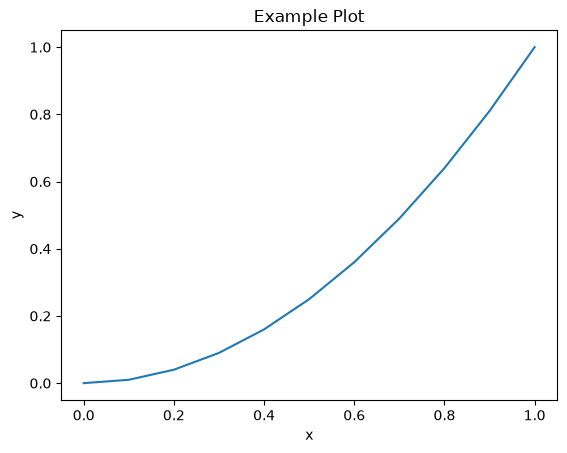
\includegraphics[width=1.0\textwidth]{Figures/Fig_Example.png}
\caption{PUT YOUR CAPTON}
\label{fig:example}
\end{figure}

% Chapter 3
\chapter{TITLE OF CHAPTER 3}\label{c:chp3}


%% =============================================================
%% Abstract in Korean (국문초록)
%% =============================================================
\newpage
\chapter*{Abstract (국문초록)}
\addcontentsline{toc}{chapter}{Abstract (국문초록)}


%% ============================================================
%% Appendix section containing supplementary material and detailed methodology
%% ============================================================
\appendix
\chapter{APPENDIX 1}\label{appendix:A}



%% ============================================================
%% Chapter: Abbreviations
%% ============================================================
\chapter*{Acronyms}\addcontentsline{toc}{chapter}{Acronyms}
\printacronyms[pages={display=all,seq/use=false},
    heading=none] % Use heading implemented in "acro" package.

%% ============================================================
%% Bibliography section
%% ============================================================
% set bibliography
\bibliographystyle{apalike}
\bibliography{references.bib}

%% ============================================================
%% Research outcomes section
%% ============================================================
% \chapter*{Research outcomes}\addcontentsline{toc}{chapter}{Research outcomes}


%% ============================================================
%% Acknowledgements section
%% ============================================================
% Hidden: this section will be initialized after Defense!
% \newpage
% \pagestyle{empty}    % no line number
% {{\textbf{Acknowledgements (감사의 글)}}}
% % {\normalsize\color{red}\bfseries \chapter*{Acknowledgements (감사의 글)}}
% \addcontentsline{toc}{chapter}{Acknowledgements}

\end{document} 